\section{Parsing and syntax trees}
\label{sect:parser_and_syntaxtrees}
The act of parsing is the process of analyzing a series of tokens and construct
a grammatical structure (syntax tree) based on a formally specified grammar. In
figure \ref{figure:parser:overview}, the parser component of a generic
compiler/interpreter is shown. 

\begin{figure}[h]
  \centering
    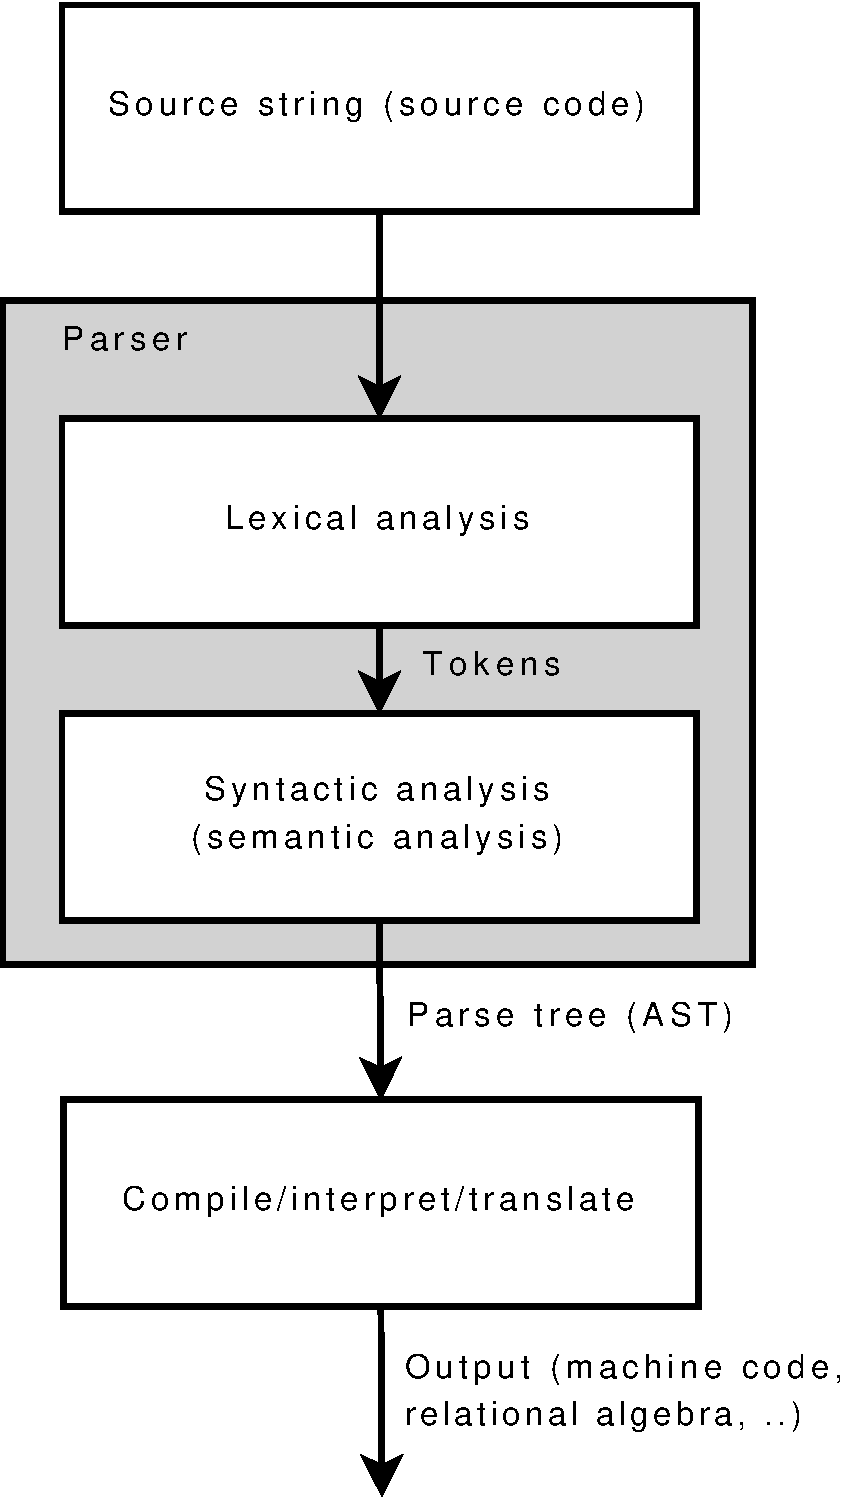
\includegraphics[scale=0.40]{diagrams/parser_overview}
  \caption{Typical compiler/interpreter data flow}
  \label{figure:parser:overview}
\end{figure}

\subsection{Common parser technologies}
There are two common types of parser technologies, \textit{top-down} and
\textit{bottom-up} parsers. As their names imply, these technologies differ in
the sense that top-down parsers will attempt to match production rules to the
input top-down, while bottom-up parsers will start at the ``bottom'' on the
terminal symbols and combine them into production rules. Often this is
implemented as a process of shift and reduce operations using stacks to hold
production rules and terminal symbols.

We refer to \cite{compiler_tech} for further in-depth information about parser
technologies, however it is important to note that typically a top-down parser
based on an LL\footnote{LL is a Left-to-right, Leftmost derivation
parser, using a top-down approach}-grammar with low token lookahead (typically
one token lookahead, aka LL(1)) will perform better and be subject to a high
number of well-defined optimizations, out of which a few are described in
\cite{compiler_tech} and \cite{DBLP:books/cu/Appel1998c}.

\subsection{Parser generators}
For large grammars, writing a parser by hand from the ground up may turn out to
be a substantial amount of work. To eliminate this, a large number of
\textit{parser generators} exist. Most of these parser generators have a very
similar set of functionality. From a formal grammar, often in a notation
similar to BNF, the parser generator will output the source code for a
complete parser for the given grammar. Ideally, the maintainability of this
generated parser could be reduced to simply changing the grammar specification,
without actually modifying the generated source code.

\begin{figure}[h]
  \centering
    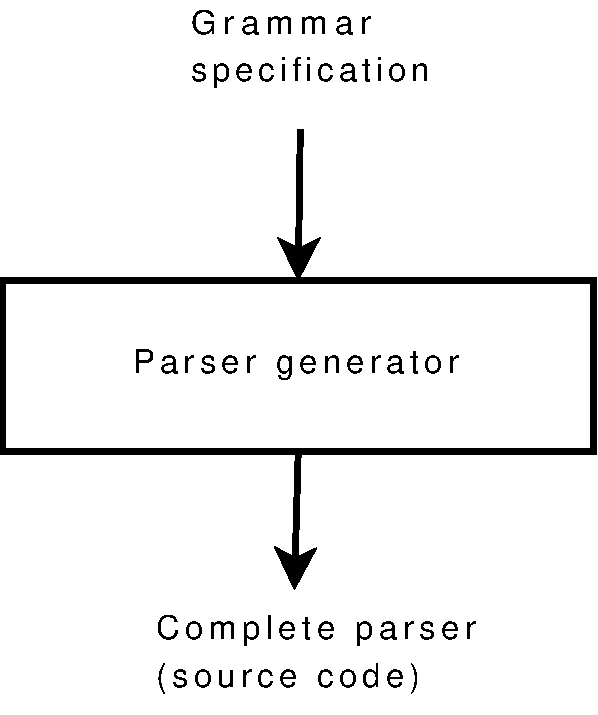
\includegraphics[scale=0.40]{diagrams/parser_generator}
  \caption{Automatic parser generation workflow}
  \label{figure:parser:generator}
\end{figure}

Several parser generators exists, covering several target languages and
overlapping in terms of functionality and features. As expected, the most
common parser generators will generate either top-down or bottom-up parsers
(described earlier in this section). Typical examples of bottom-up parser
generators are yacc (and derivatives), CUP, GOLD, and SableCC. Some popular
top-down parsers include JavaCC, ANTLR, Spirit, and Coco/R.

\marginpar{\underline{\Large TODO} \footnotesize Vi lager vel strengt tatt en LL(2 til 3) parser\ldots. Det med
LL(*) har noe med \aa~slippe \aa~ left-factor. XQuery sier heller ikke at de er LL(1) lenger\ldots det var noen
\aa r siden)} 
A comparison of some of the most popular parser generators were
made in \cite{ourselves} for the development of the XQFT Parser (see section 
\ref{sect:theory:xqftparser}), and out of these the ANTLR parser generator was
chosen. We will not reiterate the features of ANTLR in this document, however
it is important to note that ANTLR generates predicated LL(*)-parsers based on
LL-compliant grammars. This choice was made due to the XQuery BNF specification
which is claimed to be LL(1) (one token lookahead).

\subsection{The XQFT Parser project}
\label{sect:theory:xqftparser}
The XQFT Parser\cite{ourselves} was developed as a part of an academic project
at the Department of Computer and Information Science (IDI) at the Norwegian
University of Science and Technology (NTNU) throughout the autumn of 2007.

In this project the ANTLR parser generator was utilized to generate a
LL(*)-parser based on the W3C specification\cite{w3c01} for XQuery with
full-text extensions.

The output from this parser are carefully crafted abstract syntax trees which
are well suited for translation into other representations.

\subsubsection{AST construction}
The abstract syntax tree is constructed by specifying tree rewrite rules in the
grammar file (the tree rewrite rules were extensively covered in \cite{ourselves}, section
4.5). The tree consists of nodes instantiated from the
\verb!no.ntnu.xqft.parse.XQFTTree! class. To compensate for missing tokens to
determine tree context, the XQFT Parser employs the use of imaginary tokens.
These are simply tokens that do not exist in the input stream, they only have
an associated name and no specific token. These imaginary tokens are typically
used where there are no ``real'' tokens available to represent the proper
semantic or contextual meaning.

One example can be seen in figure \ref{figure:parser:imaginary_tokens_path},
where the imaginary tokens AST\_MODULE, AST\_PATHEXPR\_SGL, and AST\_STEPEXPR
have been injected into the tree.

\begin{figure}[h]
  \centering
    %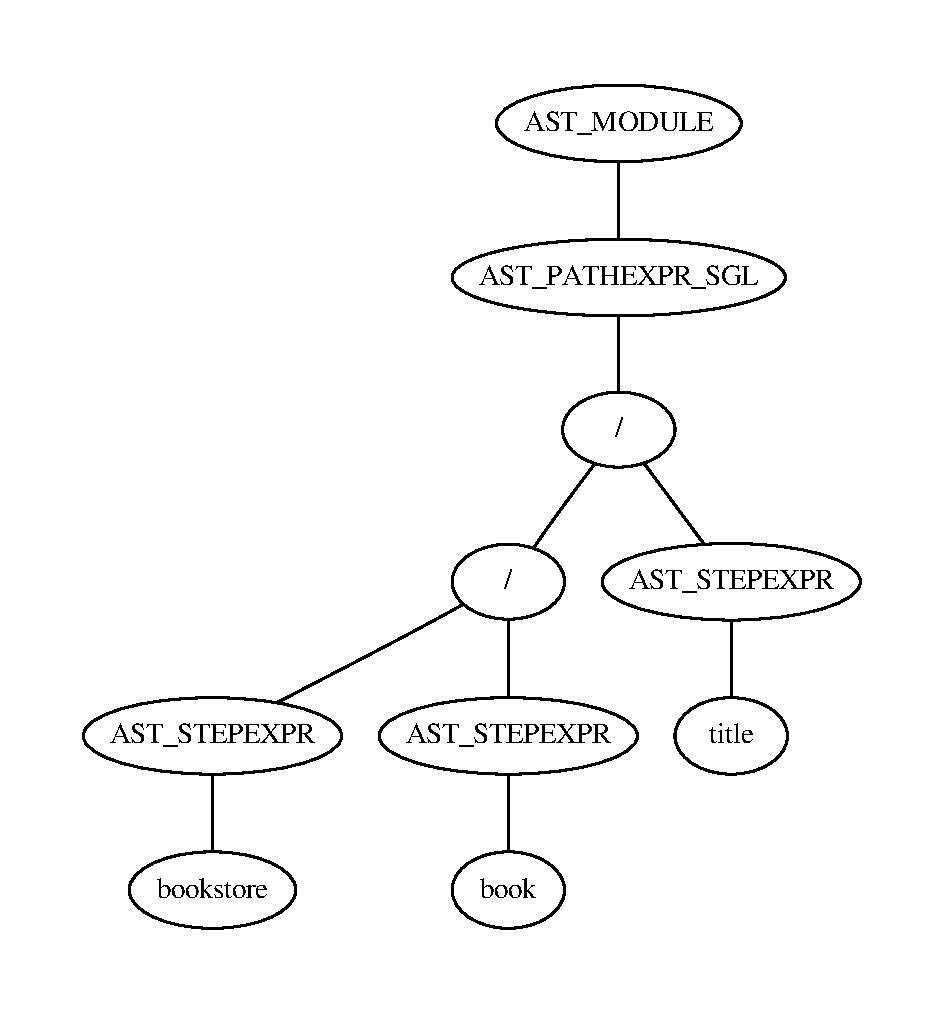
\includegraphics[scale=0.50]{diagrams/path1} 
    \underline{\textbf{\Large
    TODO: dette bildet er ikke i repository}}
  \caption{Example of injected imaginary tokens}
  \label{figure:parser:imaginary_tokens_path}
\end{figure}

The details of injection of imaginary tokens is explained in detail in
\ref{ourselves}, section 

\subsection{Tree parsing}
Tree parsing, henvise til metode eller flytte greiene fra metode og hit? Eller
noe.

\begin{itemize}
  \item Kort om forskjellige parser-teknologier
  \item Hvordan parseren vaar fungerer
  \item Hvordan ASTen ser ut\ldots kanskje nesten en egen subsection til
  dette.. iallefall i generelle trekk? hmmmmmz
  \item Syntax-tr\ae r og tre-parsing
  \item AST\_PATHEXPR\_SGL holder enkeltslash i begynnelsen av pathExprz
  \item Imagin\ae re tokens, og evt snakke om hvilke vi har lagt til i
  implementation?
\end{itemize}
